\documentclass[nofootinbib,twocolumn,showpacs,prl,superscriptaddress,secnumarabic,amssymb,nobibnotes,aps,floatfix]{revtex4}
\usepackage{graphicx}
\usepackage{hyperref}
\usepackage{amsmath}
\usepackage{dcolumn}% Align table columns on decimal point
\usepackage{bm}% bold math

%
\def\Dirac#1{#1\hskip-5pt/}
%
\begin{document}

\title{First Exclusive Measurement of Deep Virtual Compton Scattering off $^4$He: Toward the 3D tomography of nuclei}

\newcommand*{\ANL}{Argonne National Laboratory, Argonne, Illinois 60439}
\newcommand*{\ANLindex}{1}
\affiliation{\ANL}
\newcommand*{\ORSAY}{Institut de Physique Nucl\'eaire, CNRS/IN2P3 and Universit\'e Paris Sud, Orsay, France}
\newcommand*{\ORSAYindex}{2}
\affiliation{\ORSAY}
\newcommand*{\JLAB}{Thomas Jefferson National Accelerator Facility, Newport News, Virginia 23606}
\newcommand*{\JLABindex}{3}
\affiliation{\JLAB}
 
\newcommand*{\NOWJLAB}{Thomas Jefferson National Accelerator Facility, Newport News, Virginia 23606}
\newcommand*{\NOWODU}{Old Dominion University, Norfolk, Virginia 23529}
 %%%%%%%%%%%%%%% END OF Latex Macros for institute addresses  %%%%%%%%%%%%%%%%%%%%%%%%% 

\author {M.~Hattawy}
\affiliation{\ANL}
\affiliation{\ORSAY}
\author {R.~Dupr\'{e}} 
\affiliation{\ANL}
\affiliation{\ORSAY}
\author {N.A.~Baltzell} 
\affiliation{\ANL}
\affiliation{\JLAB}
\author {K.~Hafidi} 
\email[corresponding author: ]{kawtar@anl.gov}
\affiliation{\ANL}


\collaboration{The CLAS Collaboration}
\noaffiliation

%
\date{\today}
%
\begin{abstract}
We report the first exclusive measurements of deeply virtual Compton scattering 
(DVCS) off a nucleus, where all the products of the reaction including the 
recoil $^4$He nucleus were detected. The experiment was performed using the 
Jefferson Lab CEBAF Large Acceptance Spectrometer (CLAS) enhanced with a radial 
time projection chamber (RTPC) to detect the recoiling $^4$He nuclei. We 
measure large beam spin asymmetries comparable to the proton's ones and extract 
in a model independent way, the single chirally-even generalized parton 
distribution of the $^4$He nucleus. These are pioneering measurements and will 
lead the way toward the 3D imaging of the partonic structure of nuclei.  
\end{abstract}
\pacs{Valid PACS appear here}

\maketitle 

A wealth of information on the quantum chromodynamics (QCD) structure of 
hadrons lies in the correlations between the momentum and spatial degrees of 
freedom of the fundamental constituent partons, quarks and gluons. Such 
correlations are accessible via the generalized parton distributions (GPDs).  
The GPDs correspond to the coherence between quantum states of different (or 
same) helicity, longitudinal momentum, and transverse position. In an impact 
parameter space, they can be interpreted as a distribution in the transverse 
plane of partons carrying a certain longitudinal momentum 
\cite{Burkardt:2000za,Diehl:2002he,Belitsky:2002ep}. A crucial feature of GPDs 
is the access to the transverse position of partons which, combined with their 
longitudinal momentum, leads to the total angular momentum of partons 
\cite{Burkardt:2005hp}. Deep virtual Compton scattering (DVCS) corresponding to 
hard exclusive electroproduction of a real photon, which is considered as the 
cleanest probe to access GPDs and thus study the 3D imaging of nucleons and 
nuclei.

DVCS measurements have been the focus of a worldwide effort 
\cite{Stepanyan:2001sm,Airapetian,Chekanov:2003ya,Aktas:2005ty,Chen:2006na,Munoz 
Camacho:2006hx,Girod:2007aa,Gavalian:2009,Seder:2015,Pisano:2015,Jo:2015ema} 
involving several accelerator facilities such as Jefferson Lab (JLab), HERA and  
CERN. The vast majority of the experiments focused on the study of the 
nucleon's structure. The deuterium was also investigated at HERMES and JLab 
\cite{Mazouz:2007aa} mainly as a neutron target. However, studying the 3D 
imaging of the nucleon is a very important goal, understanding how these 
distributions are modified to provide the binding and structure in a nucleus is 
as fascinating of a question and an integral part of our quest of using QCD to 
explore nuclear matter. 

A DVCS process on a nuclear target differ from single nucleon scattering in 
providing access to the measure two DVCS channels. In the coherent DVCS 
channel, the target nucleus ($A$) remains intact and recoils as a whole while 
emitting a real photon ($eA \rightarrow e' A' \gamma$), allowing to measure the 
nuclear GPDs of the target. In the incoherent channel, the nucleus breaks up 
and the DVCS takes place on a bound nucleon ($N$) that emits the final photon 
($eA \rightarrow e' N' \gamma$ X), enabling the GPDs measurement of the bound 
nucleons and to study the medium modifications of the nucleons in the nuclear 
medium via the GPDs.  Figure \ref{fig:diags} illustrates the dominant mechanism 
for the coherent DVCS channel on $^4$He. At sufficiently large squared electron 
momentum transfer $Q^2$ ($= -(k-k')^{2}$) and small squared momentum transfer 
$t$ ($= (p-p')^{2}$), the QCD factorization theorem predicts that the DVCS 
handbag diagram can be factorized into two parts, hard and soft parts 
\cite{Freund_Collins,Ji_Osborne}. The hard part includes photons-quark 
interaction and it is calculable through perturbative methods, while the 
soft/non-perturbative part is parametrized in terms of GPDs, which embed the 
partonic structure of the hadron.  

\begin{figure}[tb]
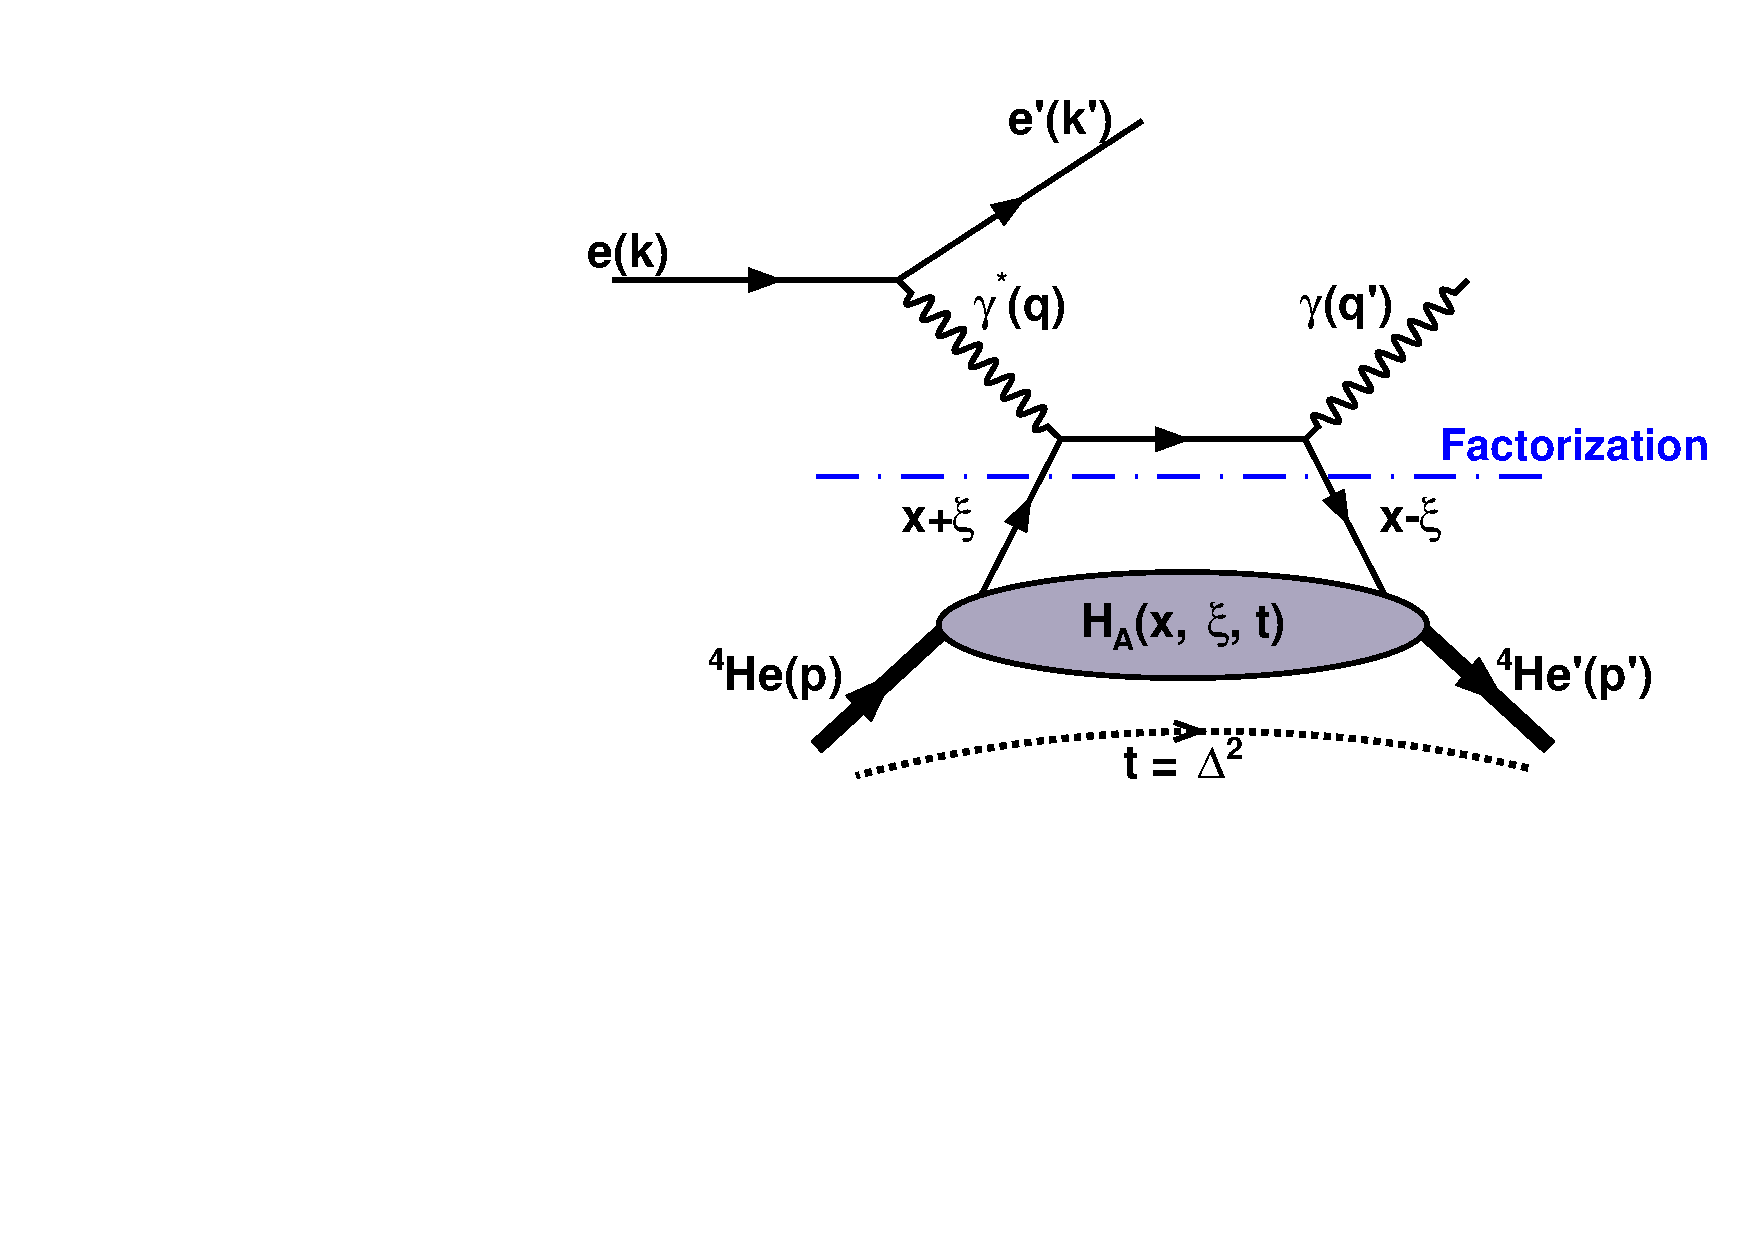
\includegraphics[width=6.5cm]{figs/DVCS_diagram.pdf}
\vspace{-0.cm}
\caption{Deep virtual Compton scattering process in the handbag approximation.}
\label{fig:diags}
\end{figure}

%introduction
The GPDs are defined for each quark flavor and gluon as matrix
elements of the light cone operators \cite{Belitsky}, describing the transition 
between the initial and final states of a hadron. The GPDs depend on two 
longitudinal momentum fraction variables ($x$, $\xi$) and on the momentum 
transfer $t$ to the target. $x$ is the average longitudinal momentum fraction 
of the parton involved in the process and $\xi$ is the longitudinal fraction of 
the momentum transfer $t$, which is related to the Bjorken variable $x_{B}$: 
$\xi\approx {{x_B}\over{2-x_B}}$, where $x_B=\frac{Q^2}{2M\nu}$ with
the proton mass $M$ and $\nu=E_e-E_{e^\prime}$. The GPDs $x$ variable cannot be 
measured experimentally in a DVCS reaction. Hence, we measure the their 
convolutions on $x$, the so-called Compton Form Factors (CFF) 
\cite{Guidal:2013rya}.  In a DVCS process, the number of GPDs needed to 
parametrize the partonic structure of a hadron depends on the different 
configurations between the spin of the hadron and the helicity direction of the 
struck quark.  Therefore, the partonic structure of spin zero nuclei, such as 
$^4He$ and $^{12}C$, is parametrized by only one GPD ($H_{A}(x,\xi,t)$) at 
leading twist, while 4 GPDs arise in the nucleon case.  In this work, we have 
chose the $^4$He nucleus as our target of interest because of it's spinless 
nature and it shows a clear EMC effect \cite{JSeely}, in addition of having a 
high density and it is a well-known few-body system.

The study of nuclear DVCS is still in its infancy due to the challenging 
detection of the low-energy recoil nuclei in fixed target experiments. Until 
very recently, the HERMES experiment \cite{Ellinghaus:2002zw} was the only one 
to measure DVCS off heavier nuclei such as $^4$He, N, Ne, Kr and Xe, where only 
the scattered electron and the real photon are detected. In this paper, we 
report the first exclusive measurements of the coherent DVCS channel off $^4$He 
where all products of the reaction are detected including the recoiling $^4$He 
nucleus. Following this exclusive measurement, the $^4$He CFF 
($\mathcal{H}_{A}$) will be extracted experimentally in a fully model 
independent way for the first time ever. The incoherent DVCS channel 
measurement from the same data set in in preparation and will reported in 
another publication. 

%experimental setup

The experiment, CLAS-EG6, took place in the experimental Hall-B of Jefferson 
laboratory (JLab) in 2009. JLab delivers, simultaneously, a nearly 100\% duty 
factor polarized electrons into three experimental Halls (A, B, C). The data 
were collected over three months via projecting a 6.064 GeV longitudinally 
polarized beam, (83$\%$ polarization), on a 6 atm gaseous $^4$He target.  The 
Hall-B Large Acceptance Spectrometer (CLAS) basic design \cite{CLAS_ref} was 
upgraded, during the CLAS-E1DVCS1 experimental run \cite{Girod:2007aa} in 2005, 
with a specially designed electromagnetic calorimeter, Inner calorimeter (IC).  
The IC has extended the photon detection acceptance of CLAS, which is 
originally from 15$^{\circ}$ to 45$^{\circ}$, to polar angle reach as minimum 
as 4$^{\circ}$. During the same experiment, a 5 Tesla solenoid was added around 
the target to shield the inner detectors from the low-energy M\o ller 
electrons.

At 6 GeV incident electron beam energy, the recoil $^4$He nuclei, from the 
coherent DVCS channel, have an average momentum (per charge) around 125 MeV/c, 
while the CLAS spectrometer detects charged particles with a threshold of 250 
MeV/c. In order to ensure the exclusivity of the our coherent DVCS channel, we 
built a small and light radial time projection chamber (RTPC) to detect 
recoiling nuclei down to energies of few MeVs. Figure~\ref{fig:RTPC} presents 
our cylindrical RTPC, which is 20 cm long and 15 cm diameter, surrounding the 
$^4$He gaseous target and being inside the available space inside the solenoid 
, with a 3 cm radial drift length. The detector was specifically calibrated for 
$^4$He nuclei using elastic scattering produced with a 1.2~GeV electron beam.


\begin{figure}[tb]
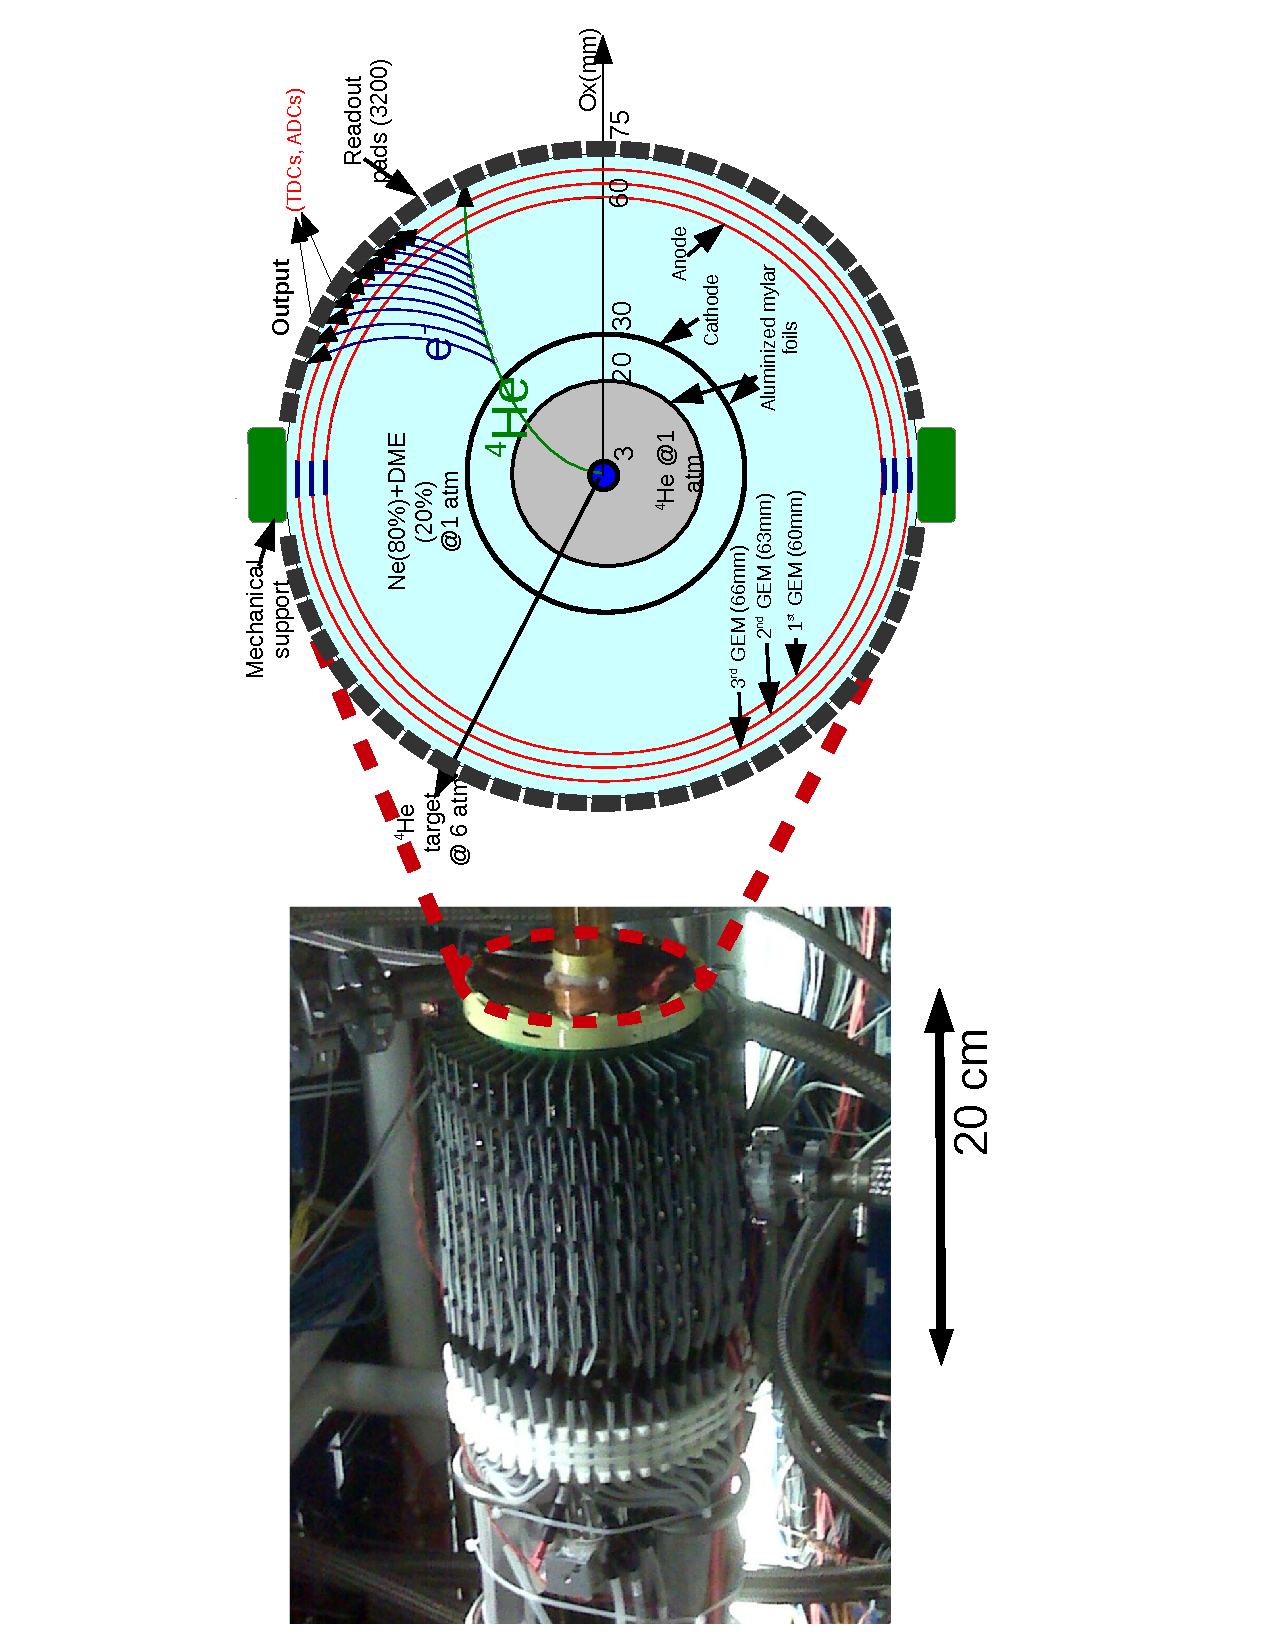
\includegraphics[width=7.0cm,angle=-90]{figs/RTPC.pdf}
\vspace{-0.9cm}
\caption{Left: A picture of the CLAS-EG6 RTPC before insertion into the 
   solenoid. Right: A cross section of the CLAS-EG6 RTPC perpendicular to the 
beam direction. An illustration of a $^4$He track originating from the 
pressurized straw target is shown along with the electrons produced in the 
drift region.}
\label{fig:RTPC}
\end{figure}

%DVCS selection
Identifying the coherent DVCS candidates is the first step of the data 
analysis. These are the events with one electron, one $^4$He, and at least one 
photon in the final state. Electrons were identified by passing the fiducial 
cuts and having signals in all the sub-detectors of CLAS spectrometer (drift 
chambers, Cherenkov counters, the standard CLAS electromagnetic calorimeter, 
and scintillators). $^4$He tracks were identified by passing all the 
geometrical, timing and quality cuts in the RTPC detector. The most energetic 
IC photon was considered as the DVCS photon candidate. Next, a 
$Q^{2}~>~[GeV^{2}/c^{2}]$ cut is applied on the DVCS candidates in order to 
ensure that the interaction occurs at the partonic level and the applicability
of the factorization in the DVCS handbag diagram. One the three final state 
particles were identified with their 3-momentum vectors, the exclusivity of the 
coherent DVCS events were ensured by applied a set of 3$\sigma$ exclusivity 
cuts. The exclusive cuts are: the co-planarity angle ($\Delta \phi$), missing 
energy, missing mass squared and missing transverse momentum in the 
$e'~^4He'~\gamma~X$ final state configuration, the missing mass squared in the 
$e'~^4He'~X$ and $e'~\gamma~X$ configurations, and finally the cone angle 
($\theta$) between the measured real photon and the missing particle in the 
$e'~^4He'~X$ configuration. Figure~\ref{fig:kin-cuts} presents four of the 
applied exclusivity cuts.

\begin{figure}[tb]
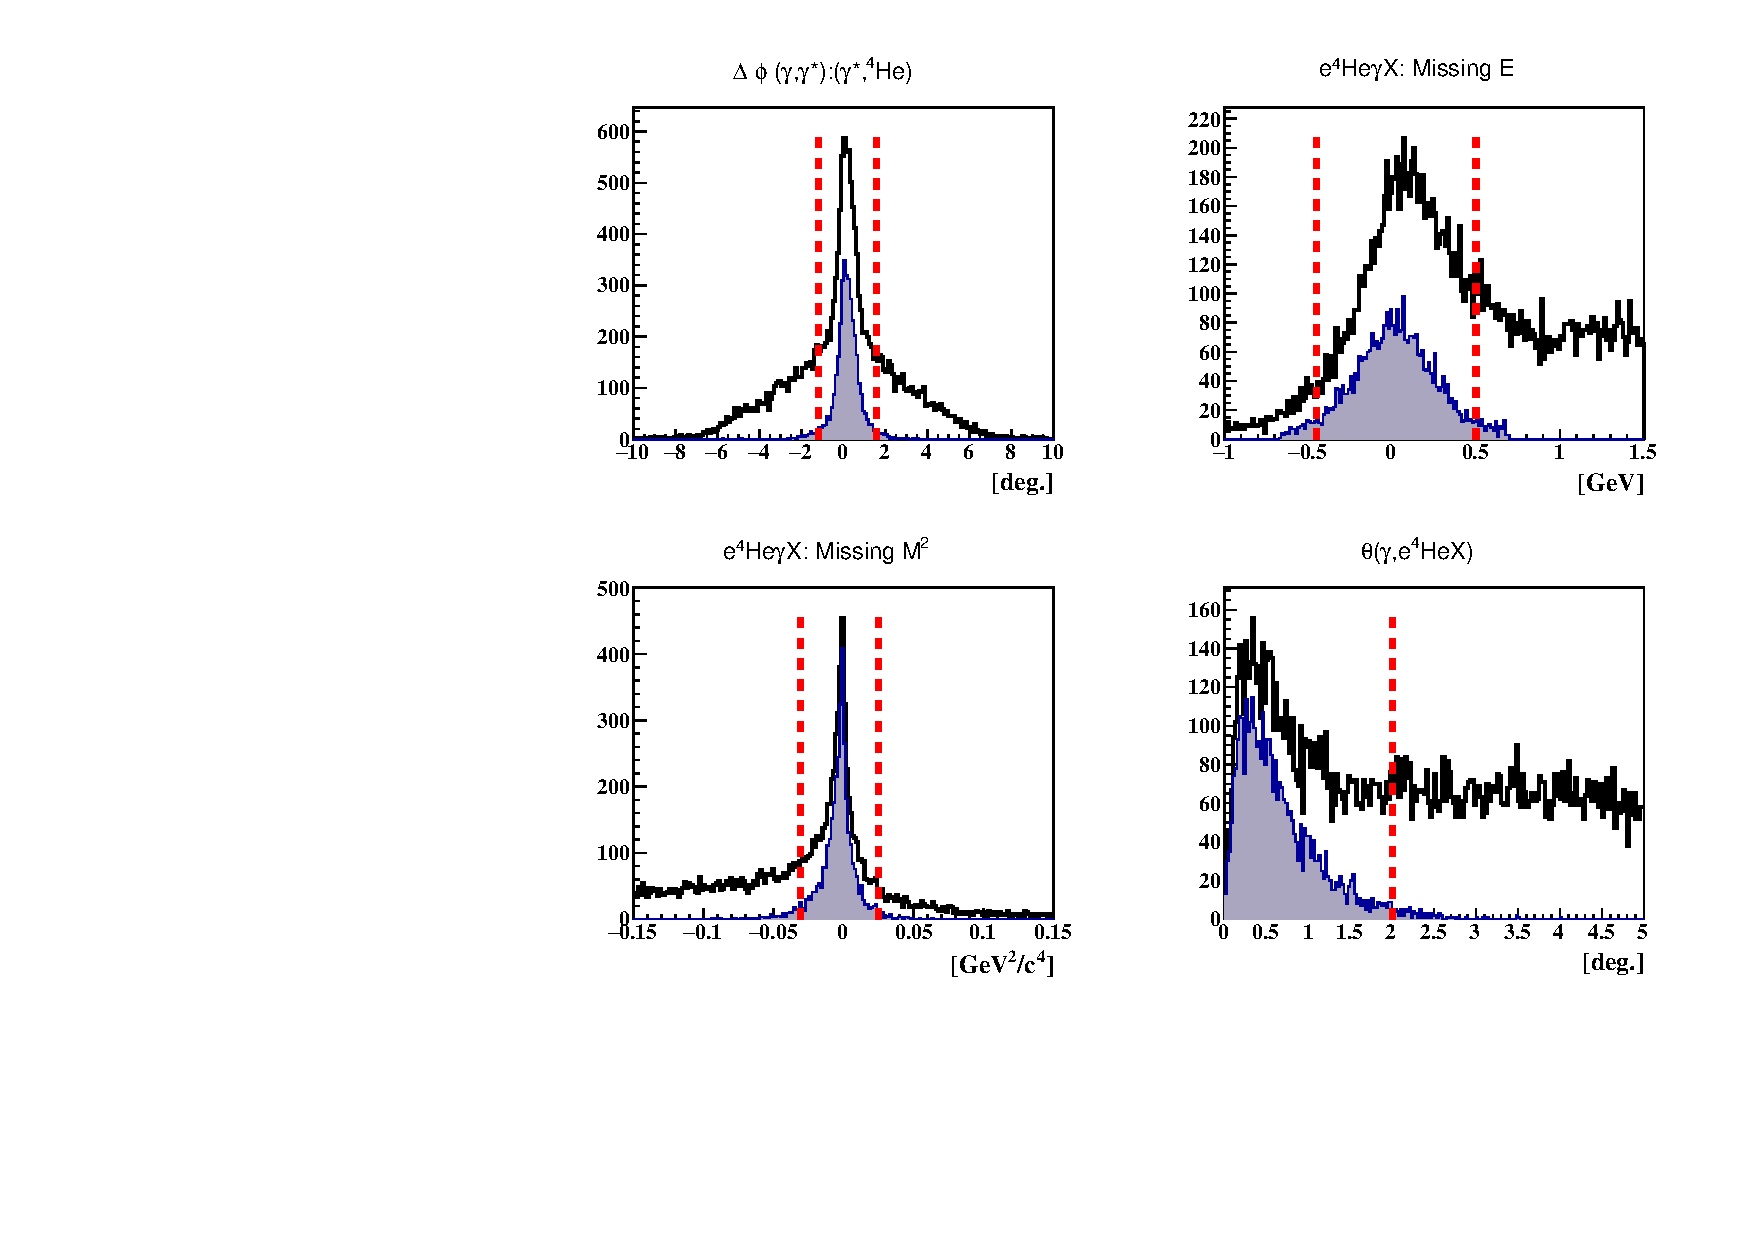
\includegraphics[width=8.9cm]{figs/coh_exc_cuts.pdf}
\caption{ The coherent DVCS exclusivity cuts. The black
distributions represent the coherent DVCS events candidate. The shaded
distributions represent the events which passed all the exclusivity cuts
except the quantity plotted. The vertical red lines represent $3\sigma$ cuts.}
\label{fig:kin-cuts}
\end{figure}

\begin{figure}[tb]
\hspace{-0.45cm}
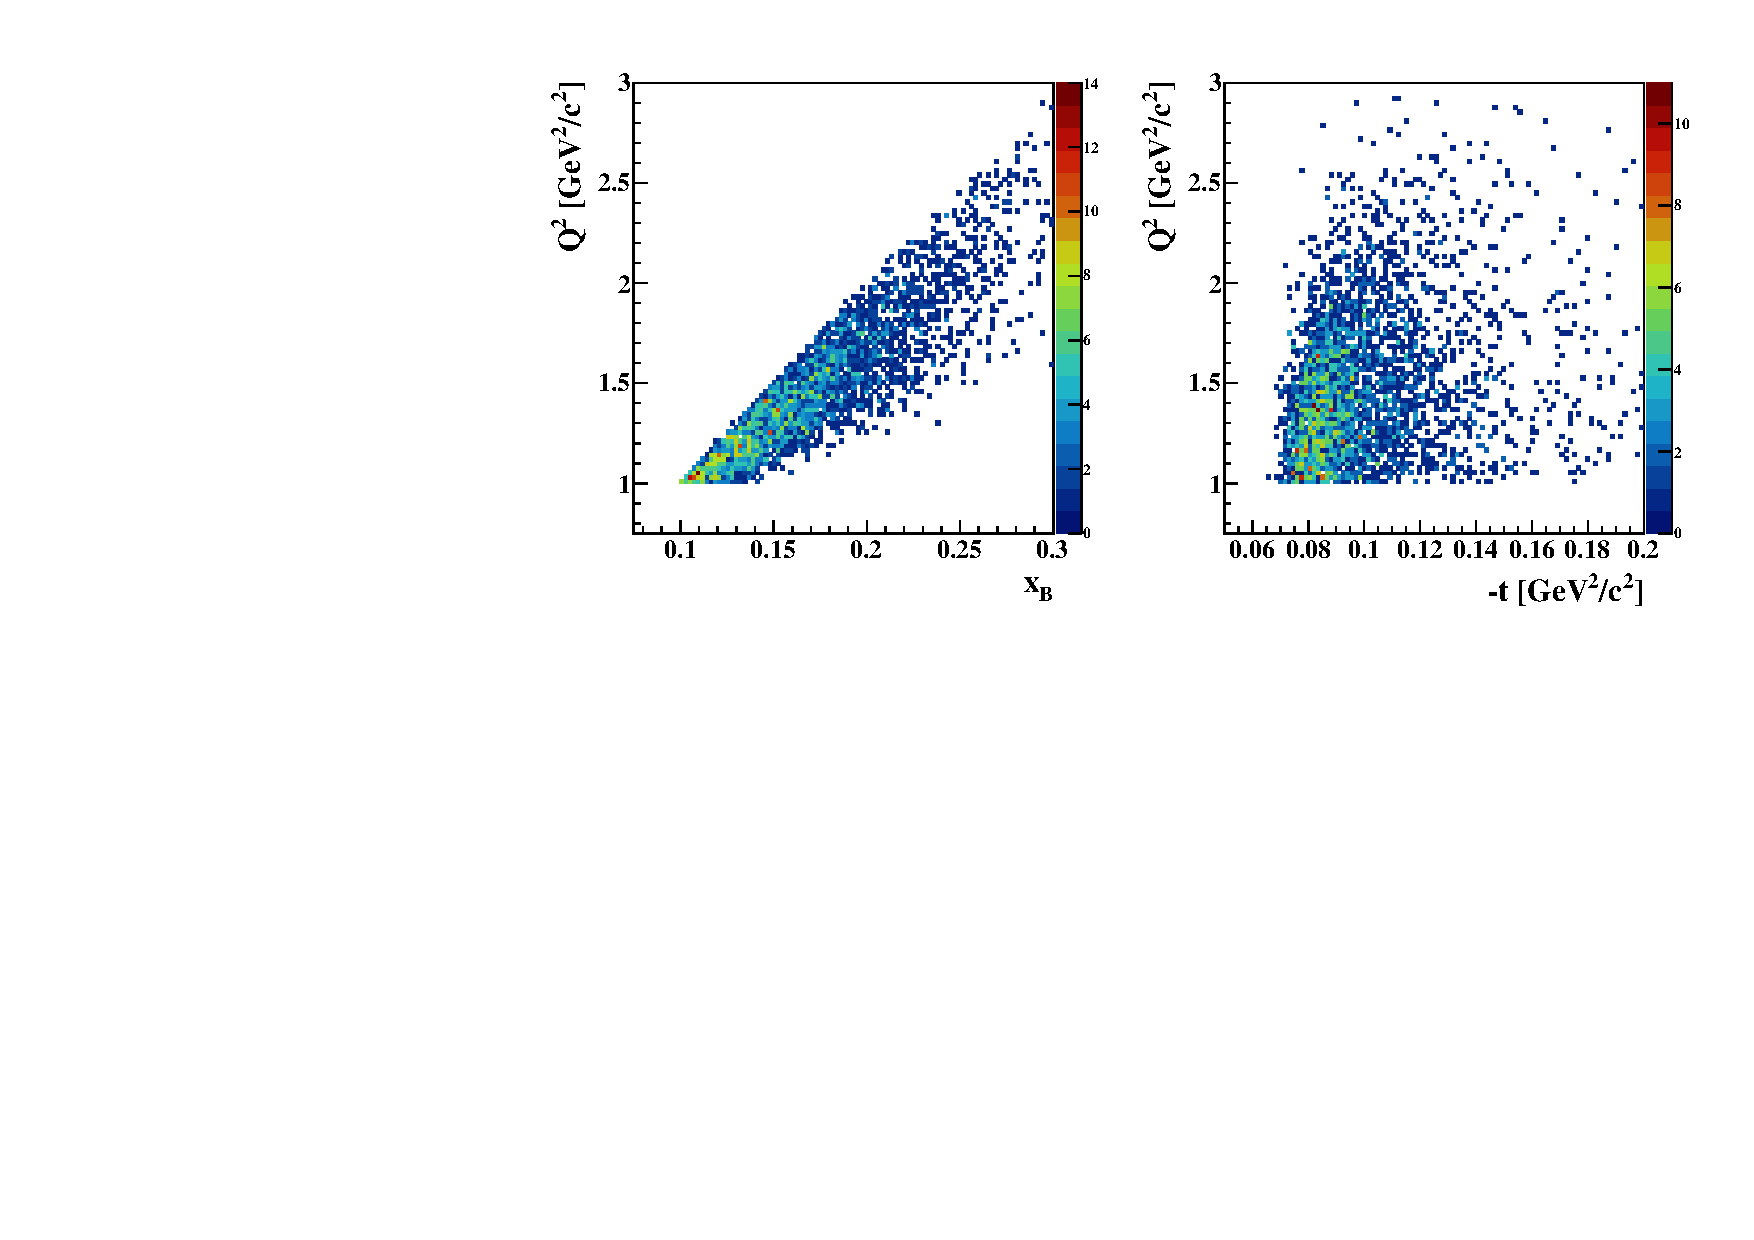
\includegraphics[width=9.0cm]{figs/Q2_xB_t_Coh.pdf}
\caption{The $Q^{2}$ as a function of $x_{B}$ (left) and the $Q^{2}$ as a 
function of $-t$ (right) for the identified coherent DVCS events after the 
exclusivity cuts.}
\label{fig:kin-coverage}
\end{figure}




%asymmetries

We identified several background contributions to the DVCS process, in 
particular accidental events and exclusive deeply virtual $\pi^0$ production 
(DV$\pi^0$P). The accidental
events where the different particles come from different events are 
suppressed by the limited phase space allowed by the exclusivity cuts. We 
estimate the accidental events to represent 4.1\% of our sample. This 
relatively large number is due to the small cross section of the DVCS. We 
evaluated this contribution by selecting events passing all our cuts but with 
particles originating from different vertices. 

Another important source of background is the deeply virtual 
$\pi^0$ production (DV$\pi^0$P), which can easily be mistaken
with DVCS when one of the two photons of the $\pi^0$ decay is produced at
low energy in the laboratory frame. To estimate the importance of
this background, we developped an event generator 
that we calibrated to match our measured experimental yield of exclusive 
$pi^0$. We used this generator together 
with a GEANT3 simulation of our detection system to estimate the ratio 
of acceptance between DV$\pi^0$P where the two photons are detected and those
where only one photon is detected and would pass our 
DVCS selection cuts. This ratio obtained from simulation is then multiplied by 
the measured yield of DV$\pi^0$P events, indicating a contamination of 2 to 4\%. 
The study of systematics errors showed that the main contributions come from 
the choice of the DVCS exclusivity cuts (8\%) and the large binning size 
(5.1\%). However added quadratically, these errors sum up to 10\% which remain 
for all bins well below the statistical errors.


The beam-spin asymmetry is measurable using a polarized lepton beam on an 
unpolarized target (U). It is convenient to use the beam-spin asymmetry as a 
DVCS observable because most of the experimental normalization and acceptance 
issues cancel out in the asymmetry ratio. It is defined as in terms of the 
cross sections as:
  \begin{equation}
  A_{LU} = \frac{d^{5}\sigma^{+} - d^{5}\sigma^{-} }
                {d^{5}\sigma^{+} + d^{5}\sigma^{-}}.
    \label{BSA_equation}
  \end{equation}
  where $d^{5}\sigma^{+}$($d^{5}\sigma^{-}$) is the DVCS differential cross section for a positive (negative) beam helicity.




In terms of the collected number of events in each beam-helicity state 
($N^{+}$, $N^{-}$), A LU can be
expressed as:

\begin{equation}
A_{LU} = \frac{1}{P_{B}} \frac{N^{+} - N^{-}}{N^{+} + N^{-} }.
\end{equation}
%
where $P_{B}$ is the beam polarization, and $N^{+}$ and $N^{-}$ are the number of events detected with positive and negative electron helicity, respectively. The statistical uncertainty of $A_{LU}$ is
%
\begin{equation}
   \sigma_{A_{LU}} = \frac{1}{P_{B}} \sqrt{ \frac{1 - (P_{B}A_{LU})^{2}}{N}}
\end{equation}
%
where $N (N^{+} + N^{-}) $ is the total number of measured events.
%


\begin{figure}[tb]
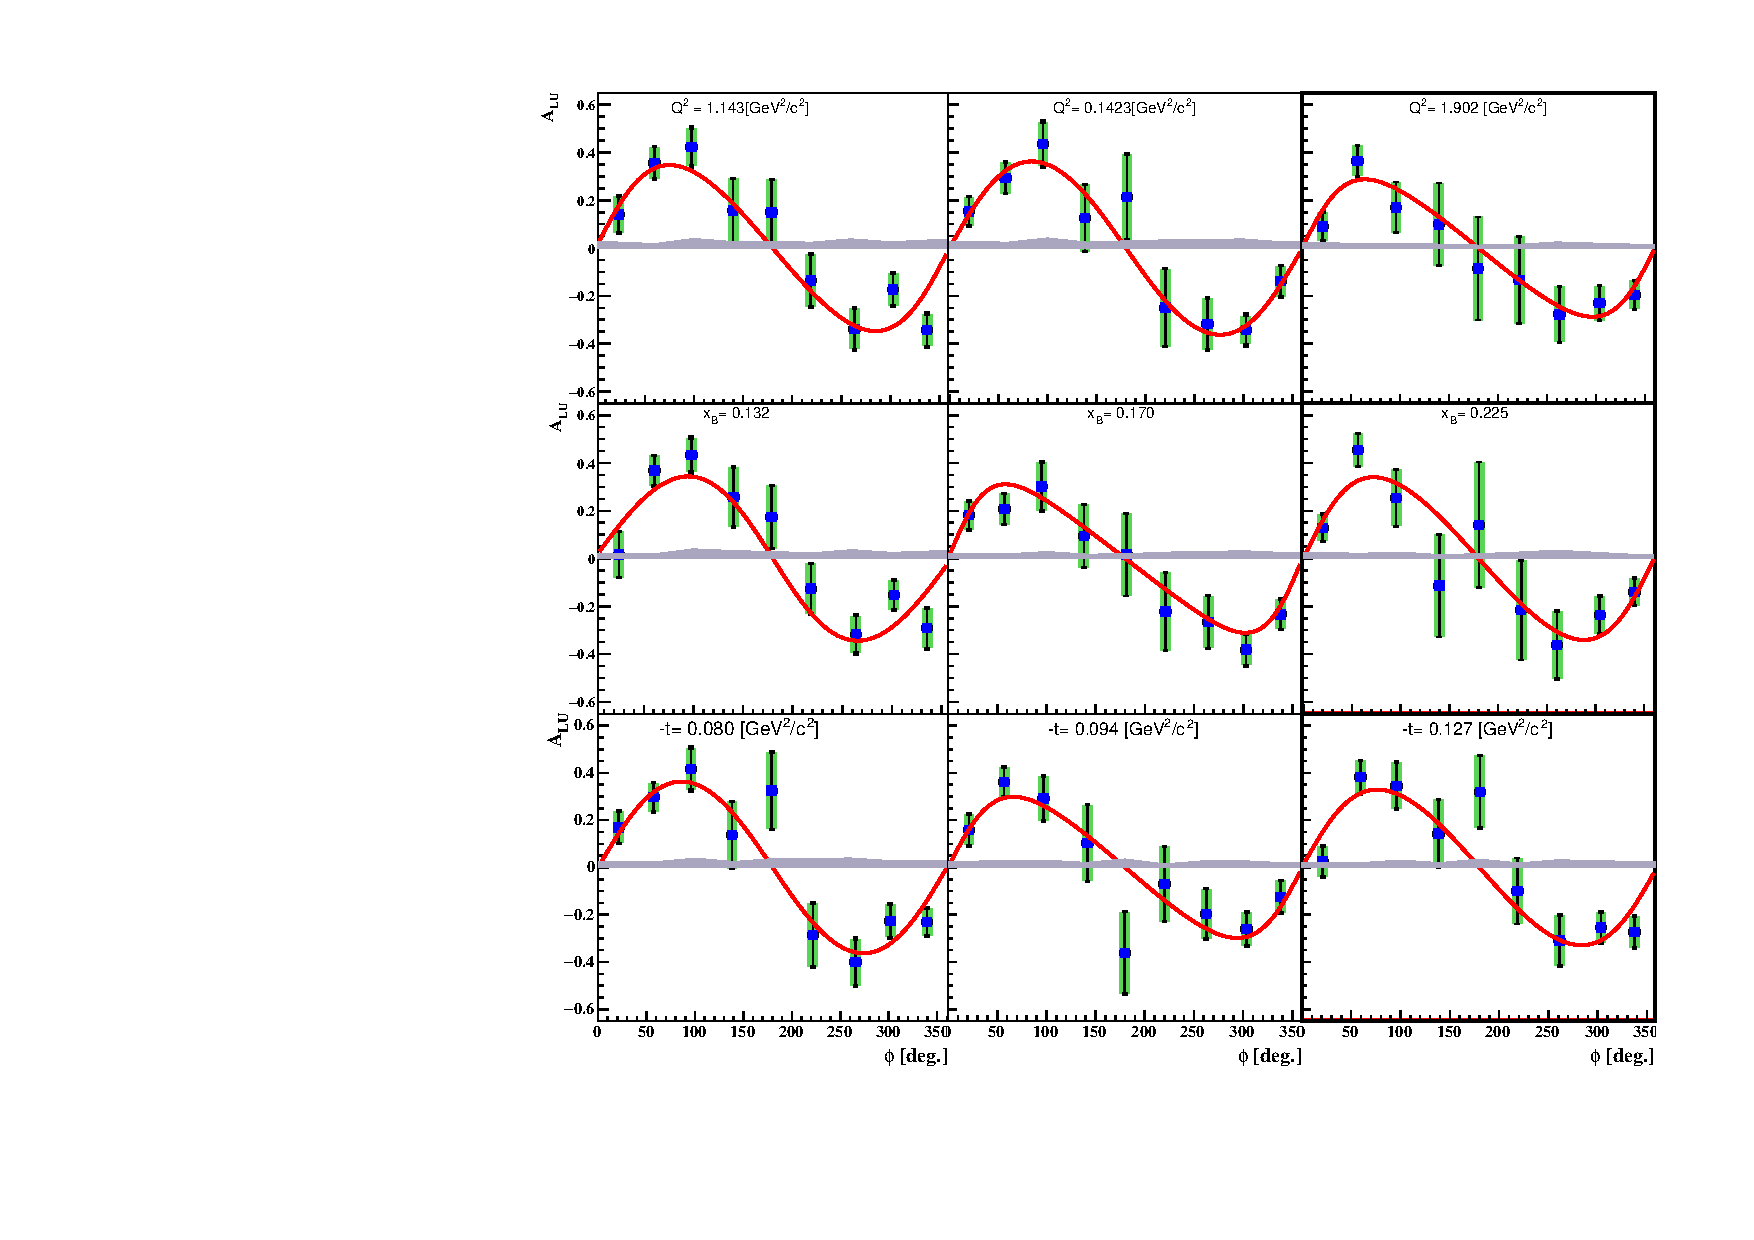
\includegraphics[width=8.9cm]{figs/coherent-ALU.pdf}
\caption{The coherent $A_{LU}$ as a function of $\phi$ in
   $Q^{2}$(top panel), $x_{B}$ (middle panel), and $-t$ (bottom panel) bins.  
   The error bars represent the statistical and the systematic uncertainties 
   added quadratically, shown on top in green are error bars representing only 
   the statistical uncertainties. The brown bands represent the systematic
uncertainties, including the normalisation systematic uncertainties. The red
curves represent fits in the form of equation \ref{eq:A_LU-coh}.}
\label{fig:alu}
\end{figure}

\begin{figure}[tb]
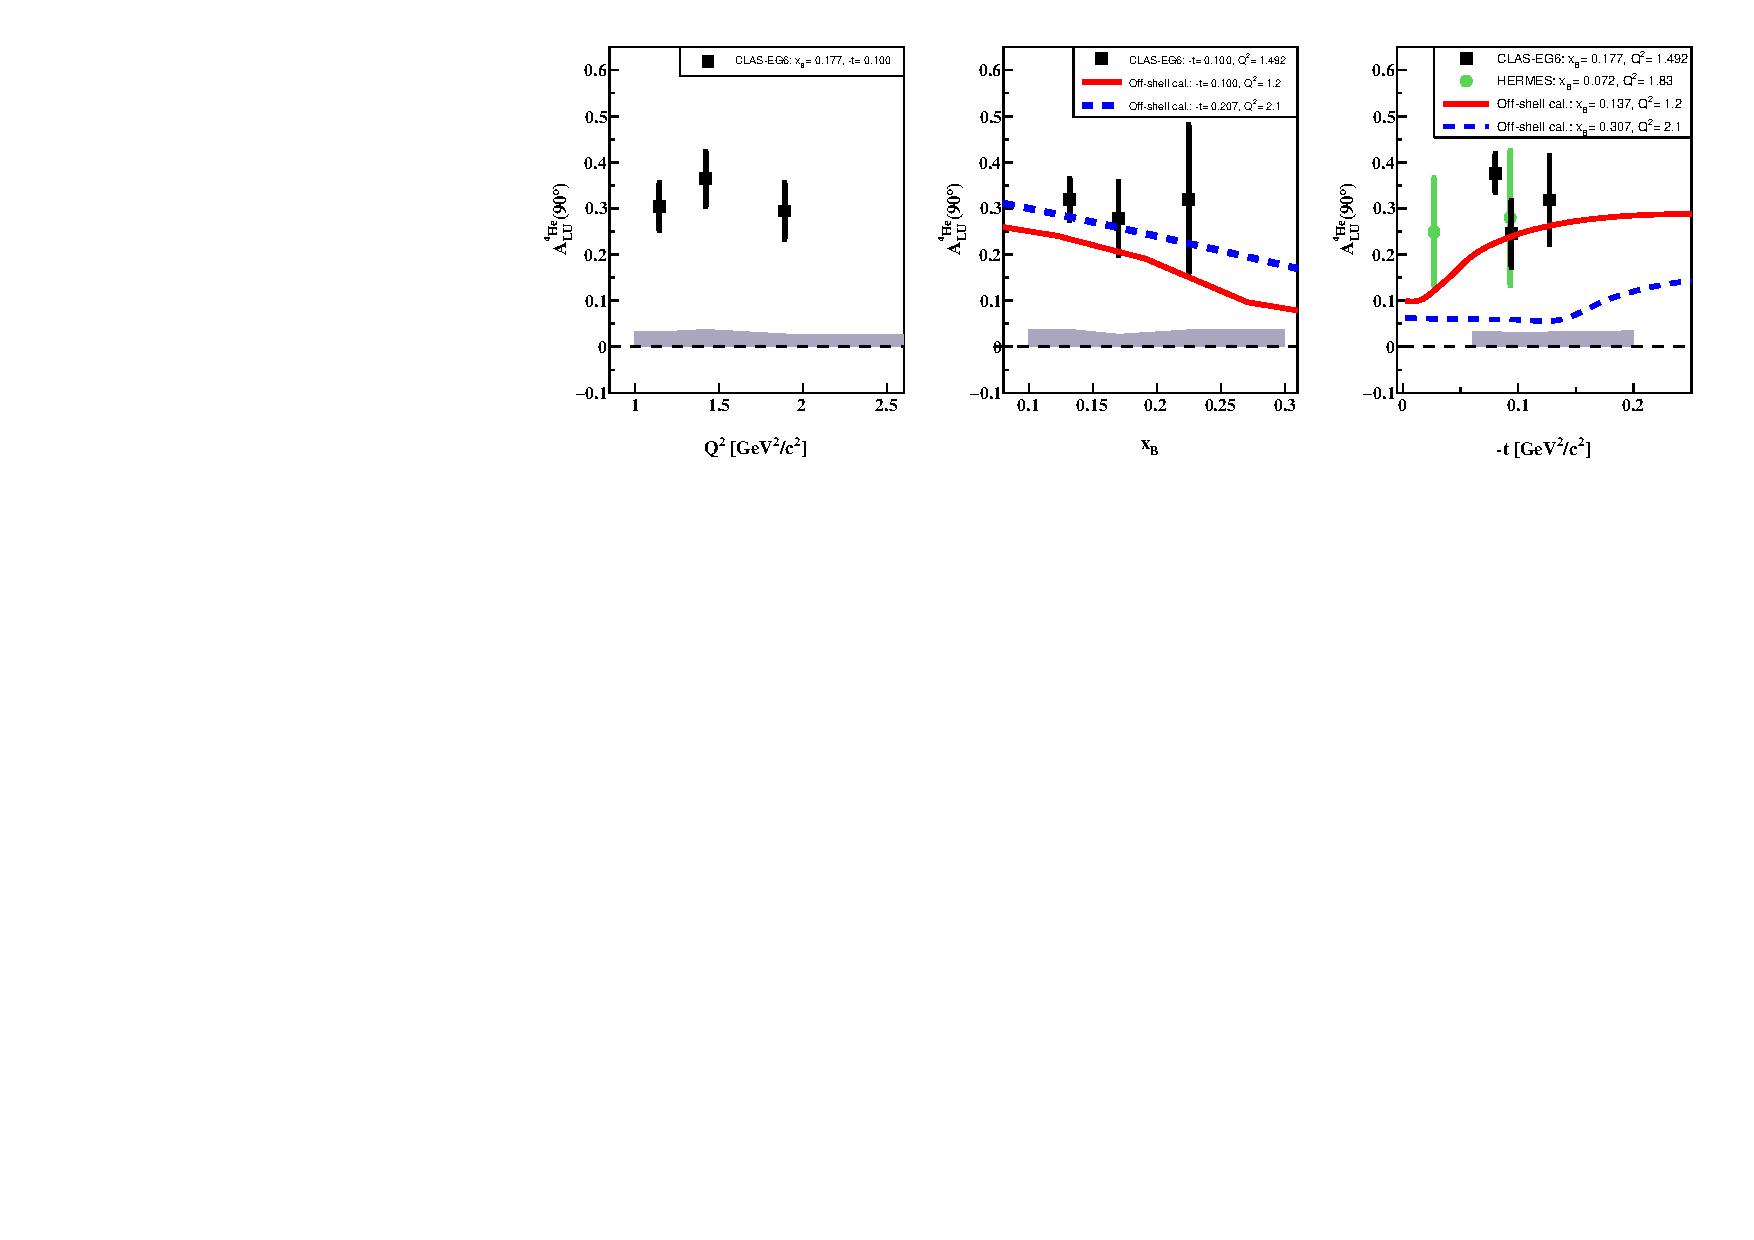
\includegraphics[width=8.9cm]{figs/coherent-ALU_90.pdf}
\vspace{-0.9cm}
\caption{}
\label{fig:alu90}
\end{figure}

%CFF
we extract the GPD $H$ in a model independent way (figure~\ref{fig:CFF_HA}).  
This is possible using the beam-spin asymmetry ($A_{LU}$) expression for 
spin-zero target at leading twist~\cite{BM_2009}:
\small
\begin{equation}
\begin{split}
A_{LU}(\phi) =~~~~~~~~~~~~~~~~~~~~~~~~~~~~~~~~~~~~~~~~~~~~~~~~~~~~~~~~~\\
 \frac{\alpha_{0}(\phi) \, \Im m(\mathcal{H}_{A})}
{\alpha_{1}(\phi) + \alpha_{2}(\phi) \, \Re e(\mathcal{H}_{A}) + \alpha_{3}(\phi) \, 
\big( 
\Re e(\mathcal{H}_{A})^{2} + \Im m(\mathcal{H}_{A})^{2} \big)}
\label{eq:A_LU-coh}
\end{split}
\end{equation}
\normalsize
%
where $\Im m(\mathcal{H}_{A})$ and $\Re e(\mathcal{H}_{A})$ are the imaginary and real parts of the CFF $\mathcal{H}_{A}$ associated to the GPD $H_A$. The $\alpha_{i}$'s are $\phi$-dependent kinematical factors that depend on the nuclear form factor $F_A$ and the independent variables $Q^2$, $x_{B}$ and $t$. These factors are simplified as:
%
\small
\begin{eqnarray}
   \alpha_0 (\phi) & = &\frac{x_{A}(1+\epsilon^2)^2}{y} S_{++}(1) \sin(\phi)\\
    \alpha_1 (\phi) & = & c_0^{BH}+c_1^{BH} \cos({\phi})+c_2^{BH} \cos(2\phi)\\ 
   \alpha_2 (\phi) & = & \frac{x_{A}(1+\epsilon^2)^2}{y}  \left( C_{++}(0) +  
C_{++}(1) cos(\phi) \right)\\
\alpha_3 (\phi) &=& \frac{x^{2}_{A}t(1+\epsilon^2)^2}{y} {\mathcal P}_1(\phi) 
{\mathcal P}_2(\phi) \cdot 2 \frac{2-2y+y^2 + \frac{\epsilon^2}{2}y^2}{1 + 
\epsilon^2}
\end{eqnarray}
\normalsize
%

Where $S{++}(1)$, $C_{++}(0)$, and $C_{++}(1)$ are the Fourier harmonics in the 
leptonic tensor. Their explicit expressions can be found in .  



\begin{figure}[tb]
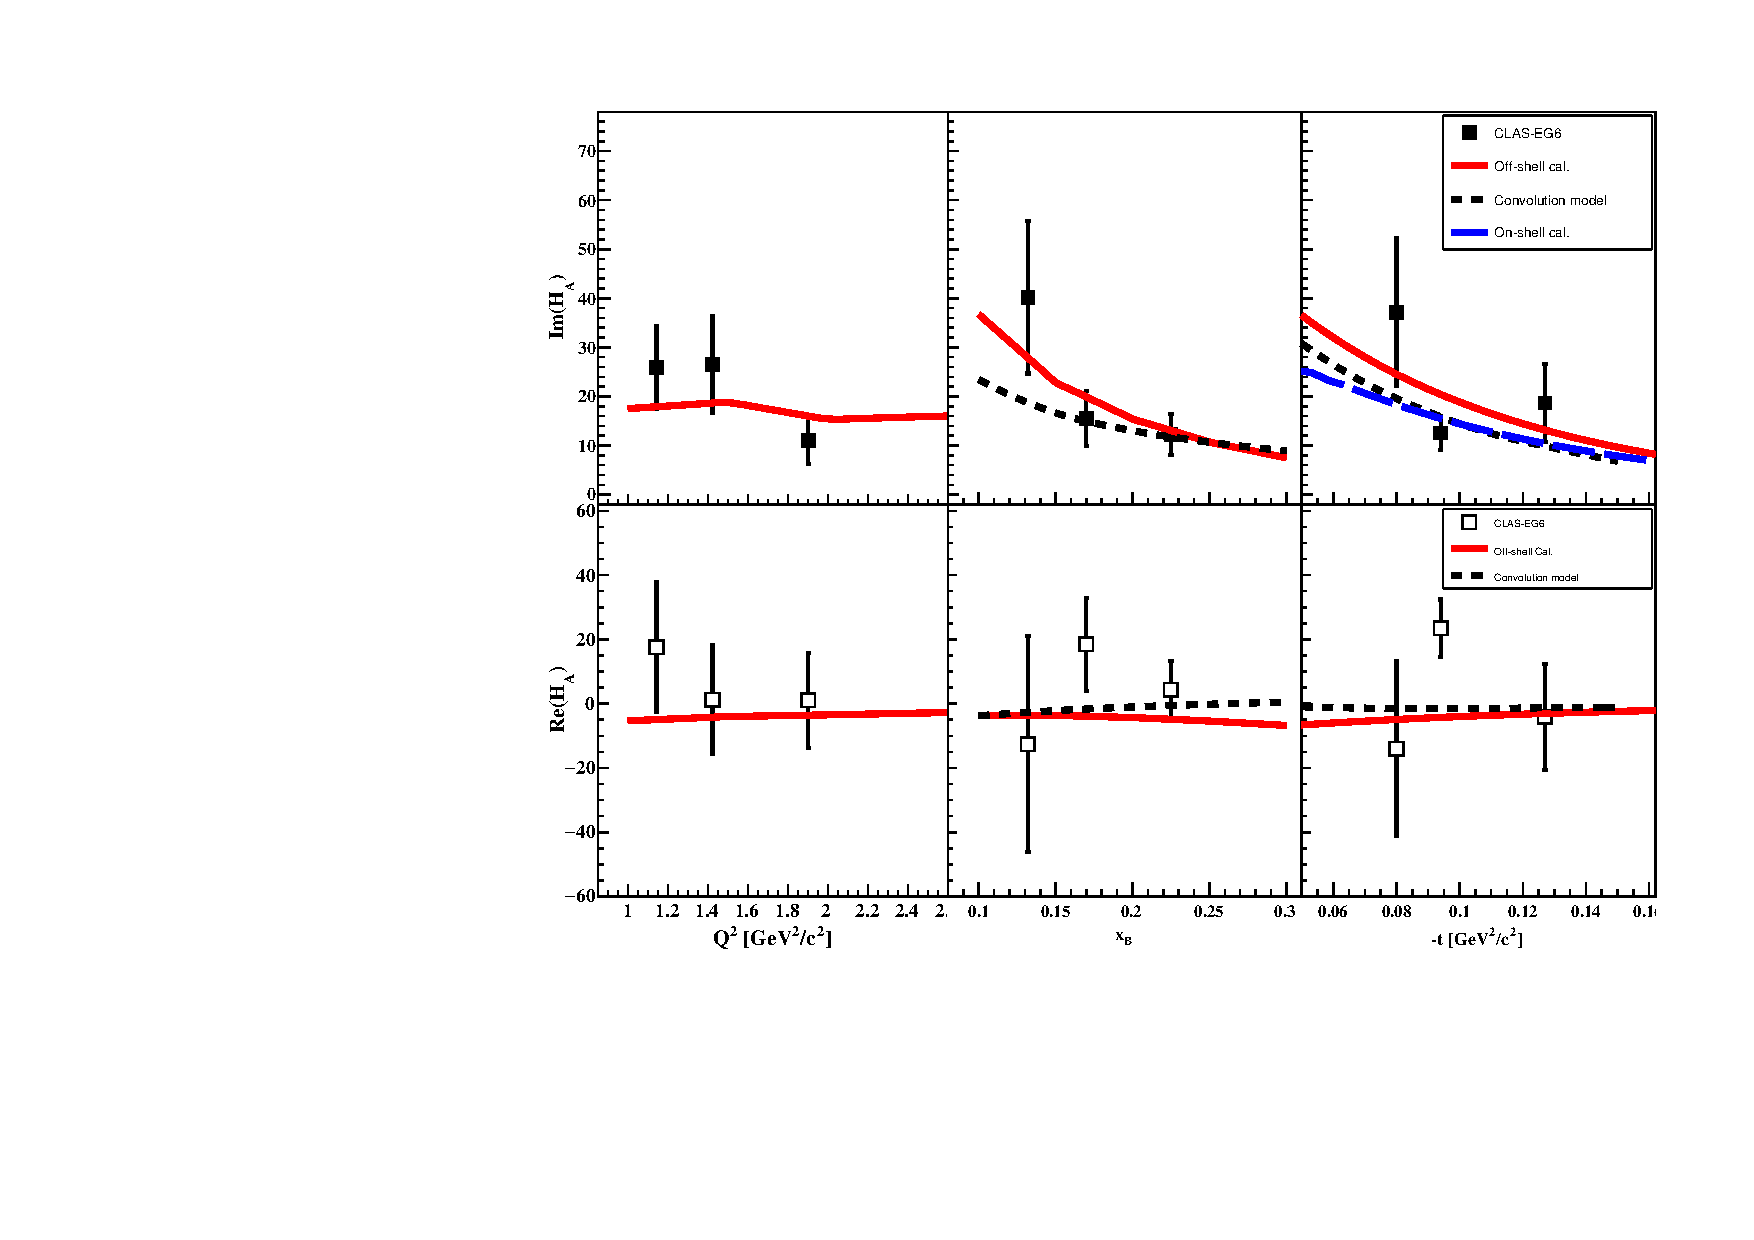
\includegraphics[width=8.9cm]{figs/Coherent_CFF.pdf}
\vspace{-0.9cm}
\caption{The model-independent extraction of the imaginary (blue points) and
real (red points) parts of the $^4$He CFF $\mathcal{H}_A$, as functions of
$Q^{2}$ (on the top right), $x_B$ (on the top left), and $t$ (on the bottom).}
\label{fig:CFF_HA}
\end{figure}

%interpretations 




%conclusion





%Acknowledgments

We thank the staff of the Accelerator and Physics Divisions
at Jefferson Lab for making this experiment possible.

\begin{thebibliography}{99}

\bibitem{Burkardt:2000za} 
  M.~Burkardt,
  Phys.\ Rev.\ D {\bf 62}, 071503 (2000)
  Erratum: [Phys.\ Rev.\ D {\bf 66}, 119903 (2002)]

\bibitem{Diehl:2002he} 
  M.~Diehl,
  Eur.\ Phys.\ J.\ C {\bf 25}, 223 (2002)
  Erratum: [Eur.\ Phys.\ J.\ C {\bf 31}, 277 (2003)]
 
\bibitem{Belitsky:2002ep} 
  A.~V.~Belitsky and D.~Mueller,
  Nucl.\ Phys.\ A {\bf 711}, 118 (2002)

\bibitem{Burkardt:2005hp} 
  M.~Burkardt,
  Phys.\ Rev.\ D {\bf 72}, 094020 (2005)

\bibitem{Stepanyan:2001sm}
S.~Stepanyan {\it et al.} [CLAS Collaboration],
Phys.\ Rev.\ Lett. {\bf 87}, 182002 (2001).

\bibitem{Airapetian}
A. Airapetian {\it et al.} [HERMES Collaboration],
Phys.\ Rev.\ Lett. {\bf 87}, 182001 (2001);
JHEP {\bf 1207}, 032 (2012);
JHEP {\bf 1006}, 019 (2010);
JHEP {\bf 0806}, 066 (2008);
Phys.\ Lett.\ B {\bf 704}, 15 (2011);
Phys.\ Rev.\  D {\bf 75}, 011103 (2007);
JHEP {\bf 0911}, 083 (2009);
Phys.\ Rev.\ C {\bf 81}, 035202 (2010);
JHEP {\bf 1210}, 042 (2012).

\bibitem{Chekanov:2003ya}
S. Chekanov {\it et al.} [ZEUS Collaboration],
Phys.\ Lett.\  B {\bf 573}, 46 (2003).

\bibitem{Aktas:2005ty}
A. Aktas {\it et al.} [H1 Collaboration],
Eur.\ Phys.\ J.\ C {\bf 44}, 1 (2005).

\bibitem{Chen:2006na} 
S.~Chen {\it et al.} [CLAS Collaboration],
Phys.\ Rev.\ Lett.\ {\bf 97}, 072002 (2006).

\bibitem{Munoz Camacho:2006hx} 
C. Mu\~noz Camacho {\it et al.} [Jefferson Lab Hall A Collaboration],
Phys.\ Rev.\ Lett. {\bf 97}, 262002 (2006).

\bibitem{Girod:2007aa} 
F.X. Girod {\it et al.} [CLAS Collaboration],
Phys.\ Rev.\ Lett. {\bf 100}, 162002 (2008).

\bibitem{Gavalian:2009} 
G. Gavalian {\it et al.} [CLAS Collaboration],
Phys.\ Rev.\ C {\bf 80}, 035206 (2009).

\bibitem{Seder:2015} 
E. Seder {\it et al.} [CLAS Collaboration],
Phys.\ Rev.\ Lett. {\bf 114}, 032001 (2015).

\bibitem{Pisano:2015} 
S.~Pisano {\it et al.} [CLAS Collaboration],
Phys.\ Rev.\ D {\bf 91}, 052014 (2015).

\bibitem{Jo:2015ema} H.~S.~Jo {\it et al.} [CLAS Collaboration],
  Phys.\ Rev.\ Lett.\  {\bf 115}, no. 21, 212003 (2015)

\bibitem{Mazouz:2007aa} 
  M.~Mazouz {\it et al.} [Jefferson Lab Hall A Collaboration],
   Phys.\ Rev.\ Lett.\  {\bf 99}, 242501 (2007)

\bibitem{Freund_Collins}
A.~Freund and J.C.~Collins, Phys.\ Rev.\ D {\bf 59}, 074009 (1998)

\bibitem{Ji_Osborne}
   X.-D.~Ji and J.~Osborne, Phys.\ Rev.\ D {\bf 58}, 094018 (1998)

\bibitem{Belitsky}
A.~V.~Belitsky and A.~V.~Radyushkin, Phys.\ Rept.\ vol. 418 (2005)

\bibitem{Guidal:2013rya}
 M.~Guidal, H.~Moutarde and M.~Vanderhaeghen,
 Rept.\ Prog.\ Phys.\  {\bf 76}, 066202 (2013)

\bibitem{JSeely}
 J. Seely {\it et al.} Phys.\ Rev.\ Lett.\ {\bf 103}, 202301 (2009)

\bibitem{CLAS_ref}
   B.A. Mecking {\it et al.}, Nucl.\ Inst.\ and Meth.\ A 503, 513 (2003).

\bibitem{Ellinghaus:2002zw} F.~Ellinghaus {\it et al.} [HERMES Collaboration],
  AIP Conf.\ Proc.\  {\bf 675}, 303 (2003)

\end{thebibliography}

\end{document}
